\documentclass{article}

% Language setting
% Replace `english' with e.g. `spanish' to change the document language
\usepackage[english]{babel}

% Set page size and margins
% Replace `letterpaper' with `a4paper' for UK/EU standard size
\usepackage[a4paper,top=2cm,bottom=2cm,left=3cm,right=3cm,marginparwidth=1.75cm]{geometry}

% Useful packages
\usepackage{amsmath}
\usepackage{listings}
\usepackage{subcaption}
\usepackage{float}
\usepackage[colorlinks=true, allcolors=blue]{hyperref}
\usepackage{xcolor}
\usepackage[utf8]{inputenc} 
\usepackage[shortlabels]{enumitem}
\usepackage{amsmath,amssymb,amsfonts,latexsym,cancel}
\usepackage{hyperref}
\usepackage{wrapfig}
\usepackage[rflt]{floatflt}
\usepackage[pdftex]{graphicx}
\usepackage{float}
\usepackage{pdfpages}
\usepackage{longtable,multirow,booktabs}
\usepackage{cite}
\usepackage{mathrsfs}
\usepackage{float}
\usepackage{wrapfig}
\usepackage[square,numbers]{natbib}
\usepackage{multicol}
\usepackage{caption}
\usepackage[]{sidecap}
\usepackage{adjustbox}
\usepackage{parskip}
\usepackage{enumitem}
\usepackage{tikz}
\usepackage{lipsum}
\usepackage[]{xcolor}
\usepackage{colortbl}
\usepackage{listings}
\usepackage{tcolorbox}
\usepackage{svg}
\usepackage{subcaption}
\usepackage{xcolor}


\title{Water simulation using examplar animation}
\author{Axel FRANZ, Romain FOURNIER, Basile SAUVAGE}
\newcommand{\commR}[1]{{\color{blue} #1}}
\newcommand{\commRI}[1]{{\color{red} #1}}


\begin{document}

%\includepdf[pages=-]{pgarde.pdf}


\begin{center}
\begin{figure}[H]
    \centering
    \begin{subfigure}[b]{0.48\linewidth}
        \centering
        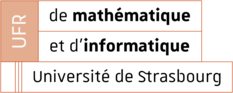
\includegraphics[height=2cm, keepaspectratio]{images/UFR.png}
    \end{subfigure}
    \hfill
    \begin{subfigure}[b]{0.48\linewidth}
        \centering
        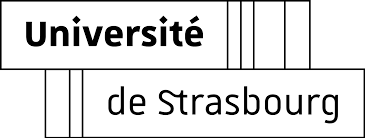
\includegraphics[height=2cm, keepaspectratio]{images/images.png}
    \end{subfigure}
\end{figure}

    \vfill

    {
	\large
	\textsc{
	       Master 1 Image et 3D
	}
    }

    \bigskip\bigskip
    \bigskip\bigskip

    {\huge Travail d'étude et de recherche}

    \bigskip\bigskip

    % Identité de l'auteur
    
    {\large Axel \textsc{FRANZ}}
    
    \vfill

    % Titre du TER : mettez un titre utile
    {
	\huge
	\textsc{
	    Procedural water rendering using tile animation
	}
    }

    \vfill
    \vfill

    \vfill

    {\large Projet encadré par}

    \medskip

    {\large Romain \textsc{FOURNIER}}
    \\
    {\large Basile \textsc{SAUVAGE}}

    \bigskip

    \bigskip

\end{center}


\newpage

\tableofcontents
\newpage

\clearpage

% Prendre du recul, parler de bruit, d'environnements, on ne peut pas stocker donc procedural dont les [...]
\begin{abstract}
Synthesizing big environments is a problem. It is very detailed so storing it as a hard value that you can read is not very viable, for some environments it would take hundreds of gigabytes hence procedural techniques rose. Water is even more subject to procedural techniques as it needs to be animated each frame to look realistic, that's why two major approaches quickly got developed, using an animated texture or displace vertices based on calculus. Both methods can work fine but it has performance issues, that's why we developed a third approach mixing both of them to create a high-performance, realistic method.
\end{abstract}

\section{Introduction}

Water simulation has always been of major interest in computer graphics. Its complex nature is the source of fascination among scientists. In order to get a water simulation in real time, you must have a fast algorithm, preferably on the GPU, and it should not have repetition artifacts. Early in the research process, two approaches have emerged : Space discretization, the Eulerian approach by Tessendorf et al\cite{tessendorf2001simulating} and Matter discretization, the Lagrangian approach by Fournier and Reeves.\cite{fournier1986simple}.


The Lagrangian approach was the first to be developed in 1986\cite{fournier1986simple}. They used a sum of Gerstner waves to compute an offset for each vertex to form a credible wave motion. Gerstner waves is one of most accurate representation of water, it's the solution of Euler's equations, they displace vertices using a tangent circular movement. This model has very good-looking results better than a sum of sines, it can show more complex form because the vertices are not only moving vertically and it has crests and depths.

The Eulerian approach appeared in 2001\cite{tessendorf2001simulating}. It uses a Fourier spectre. The spectre is an image generated on the fly with noise attached, such image can hold as many frequencies as there are pixels (usually 256*256). Each pixel has two color channels that represent the amplitude(modulus) and phase(argument) part of the frequency. This can be animated with a loop iterating through every pixel but as a result, animations can be slow to render .Using the Inverse Fourier Transform, a height map is generated and used to displace vertices on the Y-Axis.

Both methods have obvious flaws. The Eulerian approach is inefficient, it needs to generate a new spectre every frame and as the method is a texture projected onto a plane, the repetition artifacts are visible very easily. On the other hand, The Lagrangian model is also slow, it needs to compute a sum of multiple waves.

The model we propose is a mix of the benefits of both approaches. Our model uses an Eulerian approach with its height map but the map itself is Lagrangian as it is a sum of pre-calculated waves.

Our goal is to study the Fournier and Sauvage model\cite{fournier2025dynamic} with different methods to make it viable for animation. Its main use is to be easily expandable to have big plains of water without spending too much computing time.


\section{Related works}

Our work uses three already existing methods as a base. We combine and enhance them to create a realistic water model.

The first method we learned is generating colors with noise maps\cite{nvf}. The prerequisite for this method is to have 2 noise maps and a transfer function $T(x,y)$. Each noise map will give you one value. The first one will be the $x$ of the transfer function and the second one will be the $y$ with

\begin{equation}
\textbf{u} = (x,y)
\end{equation}


\label{m:1}The second method used is the composition of Gaussian noise and transfer functions using the noise map method seen previously. A Gaussian noise is a  This method is combined with method 1 as our
Gaussian noise has two color channels, they will be our \textbf{u} .
\begin{equation} \label{eq:2}
    O(\textbf{u}) = H \circ G(\textbf{u})
\end{equation}

The third method is the tiling and blending algorithm\cite{hn}. This method inputs a texture and a coordinate $\textbf{u}$. The algorithm partitions the texture, into multiple hexagons, these hexagons are combined into a single triangle with our $\textbf{u}$ inside\ref{eq:1}.

\begin{equation} \label{eq:1}
    G(\textbf{u}) = \Sigma_i{w_i(\textbf{u})E(\textbf{u})}
\end{equation}

% AJOUTER DES IMAGES DE RENDU DES 2 TYPES DE VAGUES

\section{Our Model}

\subsection{Generating the height map}
Before we understand how we animate the height map O, we must explain how to get it. The generation algorithm takes in two parameters, a profile map and an exemplar, both of them need to be pre-calculated, our algorithm doesn't generate them itself. The first part is to expand the exemplar E into an infinite texture G with the tiling and blending algorithm seen in equation\egref{eq:1}. This texture is then used to produce each UV coordinate on the plane we're projecting onto by composition of the two color channels into the profile map H as describe with equation\eqref{eq:2}.


\begin{figure}[H]
    \centering
    \begin{subfigure}[b]{0.48\linewidth}
        \centering
        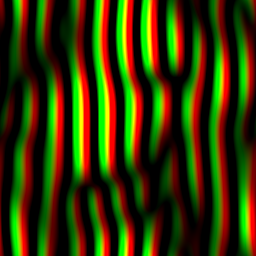
\includegraphics[height=6cm, keepaspectratio]{images/exemplar.png}
        \caption{An exemplar}
    \end{subfigure}
    \hfill
    \begin{subfigure}[b]{0.48\linewidth}
        \centering
        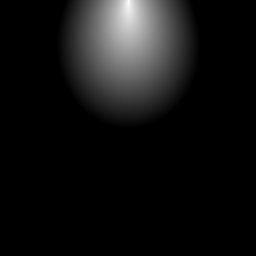
\includegraphics[height=6cm, keepaspectratio]{images/profile_map.png}
        \caption{A profile map}
    \end{subfigure}
\end{figure}

The method we used to generate a Gaussian noise is by having a color stamp with a gaussian-shaped histogram, we then apply this stamp multiple times on our texture and the resulting texture will have a gaussian-shaped histogram. This is done with a python script as it is a prerequisite.
Our profile map is also generated with external python script. They are then used as a uniform in our vertex shader.
The tiling and blending is performed purely on the GPU making use of its parallelization and being more efficient for real-time rendering.
We can compose this expanded version with the transfer function to get our final texture.


The texture $O(\textbf{u})$ is finally applied on a plane.
\begin{figure}[H]
    \centering
    \begin{subfigure}[b]{0.48\linewidth}
        \centering
        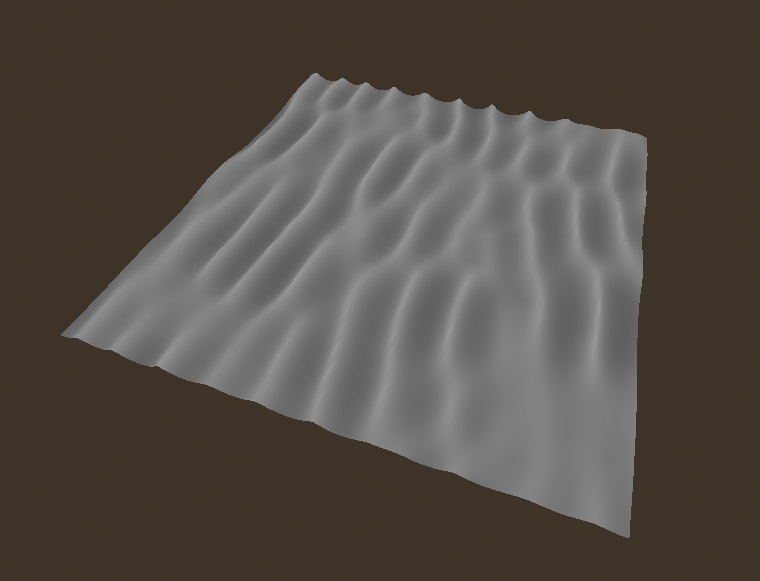
\includegraphics[height=6cm, keepaspectratio]{images/map.png}
        \caption{A height map}
    \end{subfigure}
    \hfill
    \begin{subfigure}[b]{0.48\linewidth}
        \centering
        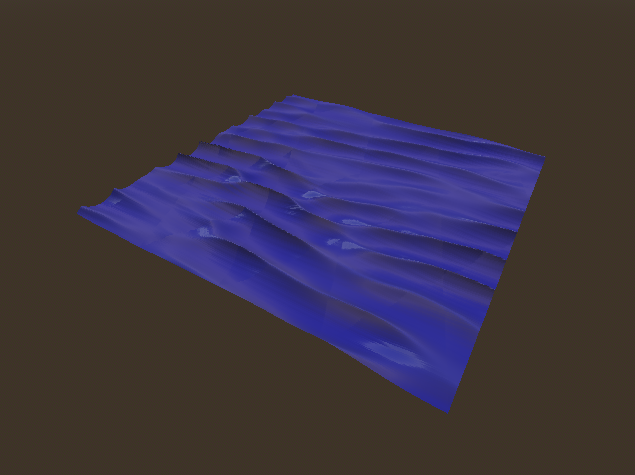
\includegraphics[height=6cm, keepaspectratio]{images/eau.png}
        \caption{Water generated with our modem}
    \end{subfigure}
\end{figure}

\subsection{Animating the height map}
As we saw previously, generating our height map has 3 main parts, you select the hexagons for the tiling and blending, you expand the examplar E onto the infinite texture G and then you compose with the transfer function H. We tried animating each part of the algorithm to see what could be used or not, the steps are show in the figure below.
\begin{figure}[H]\label{sch:1}
    \centering
    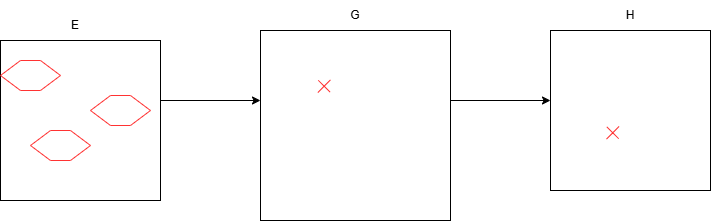
\includegraphics[width=15cm,keepaspectratio]{images/schema.png}
    \caption{Interaction between the textures}
\end{figure}

\subsubsection{Input approach}
We tried animating the exemplar but quickly realized it was impossible. The input of our program is an already generated exemplar. It takes about 4 seconds to generate thus it can't be recalculated every frame but if a method to quickly generate a gaussian noise is found, this method can be developed and it should look good. You can try to develop like Tessendorf\cite{tessendorf2001simulating} where the map is generated quickly with pure parallelism on the GPU whereas our gaussian noise is generated sequentially on the CPU.
\subsubsection{UV approach} 
The first and most naive approach we tried is to create a copy of \textbf{u} via a time-parametrized offset to change its coordinate (but not visually). It changes the equation of $O(\textbf{u})$\ref{eq:2} into

\begin{equation}
    O(\textbf{u)} = H \circ G(\textbf{u}+\textbf{o}(t))
\end{equation}.

The offset used was 

\begin{equation}
    \textbf{o}(t) = \begin{bmatrix} t/10 & 0\end{bmatrix}
\end{equation}

This modification results in a sliding artifact, where the ocean seems to be translated and not animated.

\subsubsection{Rotating approach}

Rotating the infinite generated texture H was our next try. The examplar is not a uniform texture so moving it after getting our \textbf{u} felt like something random and wave-looking like.

The equation\ref{eq:1} was changed into 

\begin{equation}
    O(\textbf{u})=H\circ (R(t)\cdot G(\textbf{u}))
\end{equation}

with $R(t)$ the rotation matrix with the angle t.

This method didn't work as expected, there were easily seeable repetition artifacts.

\subsubsection{Tiling approach}
The last and working approach tried with this model was to change the tile used by the tiling and blending, they can be seen in figure 4 as little hexagons\ref{sch:1}, with an offset through time variation, we call it $\textbf{o}(t)$.
The offset we used is just

\begin{equation} \label{eq:3}
\textbf{o}(t) = \begin{bmatrix} t/10 & 0\end{bmatrix}
\end{equation}
The equation\ref{eq:1} is changed into
\begin{equation} \label{eq:4}
G(\textbf{u}) = \Sigma_i{w_i(\textbf{u})E(\textbf{u}+\textbf{o}(t))}
\end{equation}

This method is as fast as the others and produce better results, it does not have the slider artifact nor the repetition artifact.
\section{Results}

The tiling method was the one kept for the final version of the model. It produced the better results. \ref{video:1}

It had some artifacts from the tiling and blending, the grid used for the space discretization is visible. It should come from the animation giving non-smooth edges but it has not be fixed.


\begin{figure}[H]
    \centering
    \begin{subfigure}[b]{0.48\linewidth}
        \centering
        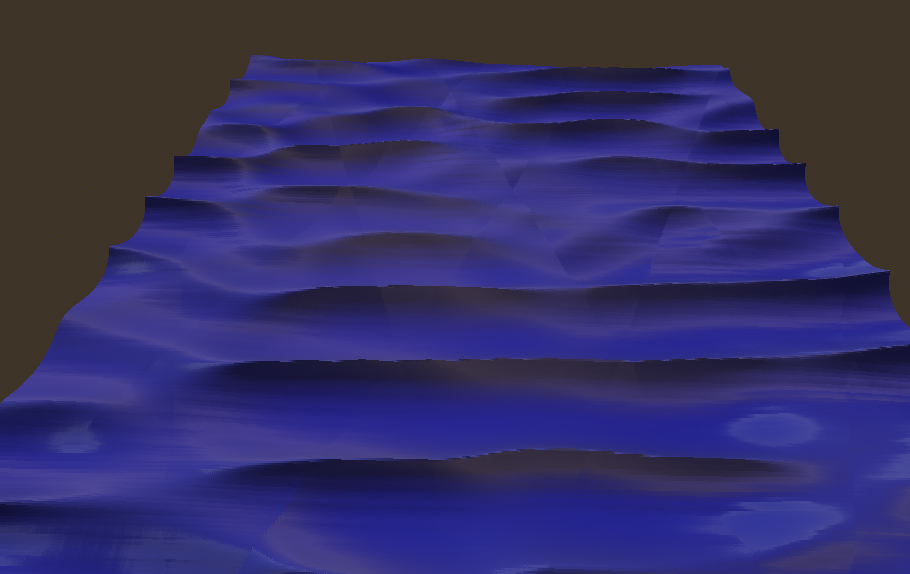
\includegraphics[height=4.5cm, keepaspectratio]{images/anoh.png}
    \end{subfigure}
    \hfill
    \begin{subfigure}[b]{0.48\linewidth}
        \centering
        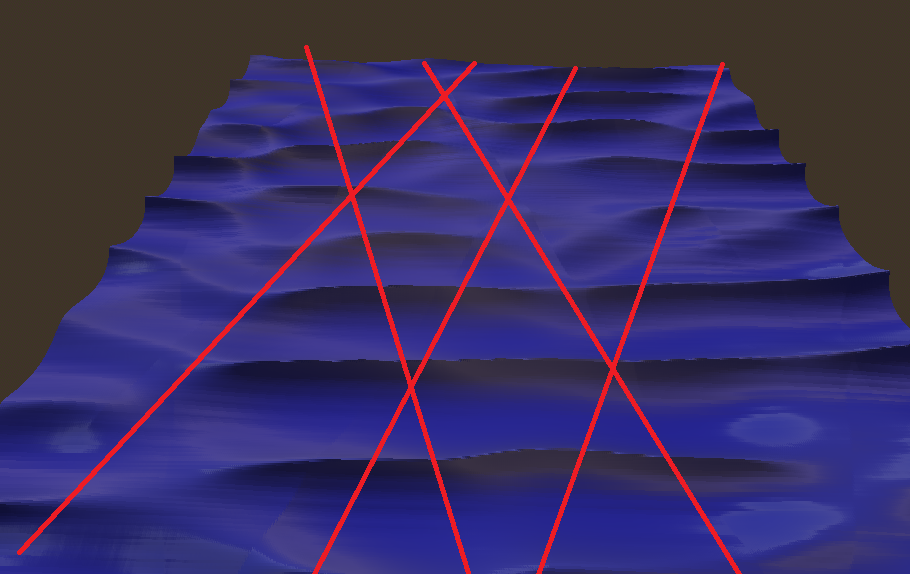
\includegraphics[height=4.5cm, keepaspectratio]{images/aoh.png}
    \end{subfigure}
    \caption{Artifacts visible on the left and highlighted on the right}
\end{figure}

A new frame was generated every 6.90ms on a RTX 4070 Portable, it averages 410FPS with a 512 * 512 plane which is more than enough for real-time rendering.


\begin{tabular}{cc}
Strengths & Weaknesses\\
 \hline
 Fast to render & Tiling and Blending artifacts\\
Easy to implement &  Need to implement on the CPU for buoyancy\\
Can easily be applied to big environments& Need to have an already generated exemplar and profile map\\
    \end{tabular}



\bibliographystyle{alpha}
\bibliography{sample}

\section{Appendix}

\subsection{Link to a video showing the water} \label{video:1}
\href{https://youtu.be/tlrDJOwRbNo}{https://youtu.be/tlrDJOwRbNo}

\subsection{Link to the Godot project repository}
\href{https://github.com/AxelFranz/TERFoam}{https://github.com/AxelFranz/TERFoam}

\subsection{Code used in Godot Engine}
\begin{lstlisting}
shader_type spatial;
//render_mode unshaded;
uniform bool printgrid = false;
uniform sampler2D uSamplerAlbedo : repeat_enable, filter_linear_mipmap;
uniform sampler2D uSamplerTransfer : repeat_disable;

#define ANIM_TUILE
//#define ANIM_ROTA
//#define ANIM_UV

vec2 hash(in ivec2 p) {
	mat2 hashMat = mat2(
		vec2(127.1, 269.5),
		vec2(311.7, 183.3)
	);

	vec2 q = hashMat * vec2(p);
	q[0] = sin(q[0]);
	q[1] = sin(q[1]);
	q *= 43758.5453;
	return vec2(q[0] - floor(q[0]), q[1] - floor(q[1]));
}

void TriangleGrid(in vec2 p_uv, inout vec3 Bi, inout ivec2 vertex1, inout ivec2 vertex2, inout ivec2 vertex3)
{
	vec2 uv = p_uv * 2.0 * sqrt(3.0);

	mat2 gridToSkewedGrid = mat2(
		vec2 (1.0, -0.57735027),
		vec2 (0.0, 01.15470054)
	);

	vec2 skewedCoord = gridToSkewedGrid * uv;
	vec2 baseId = vec2(floor(skewedCoord[0]), floor(skewedCoord[1]));
	vec3 temp = vec3(skewedCoord[0] - baseId[0], skewedCoord[1] - baseId[1], 0.0);
	temp[2] = 1.0 - temp[0] - temp[1];

	if (temp[2] > 0.0)
	{
		Bi = vec3(temp[2], temp[1], temp[0]);
		ivec2 ibaseId = ivec2(baseId);
		vertex1 = ibaseId;
		vertex2 = ibaseId + ivec2(0, 1);
		vertex3 = ibaseId + ivec2(1, 0);
	}
	else
	{
		Bi = vec3(-temp[2], 1.0 - temp[1], 1.0 - temp[0]);
		ivec2 ibaseId = ivec2(baseId);
		vertex1 = ibaseId + ivec2(1, 1);
		vertex2 = ibaseId + ivec2(1, 0);
		vertex3 = ibaseId + ivec2(0, 1);
	}
}

vec3 tiling_n_blending(vec2 uv, sampler2D tex, vec2 duvdx, vec2 duvdy) {
	vec3 B;
	ivec2 vertex1, vertex2, vertex3;
	TriangleGrid(uv, B,	vertex1, vertex2, vertex3);

	// Assign random offset to each triangle vertex
    // Hash = centre de la tuile et UV ou on est
    // 3e approche : bouger uv1,2,3
    #ifdef ANIM_TUILE
    vec2 uv1 = uv + hash(vertex1) * TIME/10.f ;
	vec2 uv2 = uv + hash(vertex2) * TIME/10.f;
	vec2 uv3 = uv + hash(vertex3) * TIME/10.f;
    #else
    vec2 uv1 = uv + hash(vertex1);
	vec2 uv2 = uv + hash(vertex2);
	vec2 uv3 = uv + hash(vertex3);
    #endif
	vec3 e = textureLod(tex, uv, 100).rgb;

	vec3 t1 = textureGrad(tex, uv1, duvdx, duvdy).rgb;
    vec3 t2 = textureGrad(tex, uv2, duvdx, duvdy).rgb;
    vec3 t3 = textureGrad(tex, uv3, duvdx, duvdy).rgb;

    vec3 W = vec3(0);
	W[0] = B[0] / sqrt(B[0]*B[0] + B[1]*B[1] + B[2]*B[2]);
	W[1] = B[1] / sqrt(B[0]*B[0] + B[1]*B[1] + B[2]*B[2]);
	W[2] = B[2] / sqrt(B[0]*B[0] + B[1]*B[1] + B[2]*B[2]);
	
	if (printgrid) {
		vec3[] c = {vec3(1, 0, 0), vec3(0, 1, 0), vec3(0, 0, 1)};
		e = vec3(1.0/3.0);
		t1 = c[(vertex1.x + 2 * vertex1.y) % 3]; 
		t2 = c[(vertex2.x + 2 * vertex2.y) % 3]; 
		t3 = c[(vertex3.x + 2 * vertex3.y) % 3]; 
	}

    vec3 P = W[0] * (t1 - e) + W[1] * (t2 - e) + W[2] * (t3 - e) + e;

    return P;
}

varying vec2 UVmodif;
varying float h;

float random (vec2 uv) {
    return fract(sin(dot(uv.xy,
        vec2(12.9898,78.233))) * 43758.5453123);
}

vec2 rota(float angle, vec2 point) {
    angle = angle * PI / 180.f;
    
    mat2 rot = mat2(vec2(cos(angle),-sin(angle)),vec2(sin(angle),cos(angle)));
    
    return rot * point;
    
}

void vertex() {
	// Call.ed for every vertex the material is visible on.
#ifdef ANIM_UV
    UV.x += TIME/30.f;
#endif    
    vec2 duvdx = vec2(0.01, 0.0);
    vec2 duvdy = vec2(0.0, 0.01);
    vec2 res = tiling_n_blending(UV,uSamplerAlbedo, duvdx, duvdy).xy; // Le bruit gaussien se génère là
    res = normalize(res) * tanh(length(res));
    #ifdef ANIM_ROTA
    res = rota(TIME*360.f,res);
    #endif
    h = texture(uSamplerTransfer, res * 0.5 + 0.5).r / (2.0 * PI * 5.0);
    VERTEX.y += h;
}   

void fragment() {
    vec2 res = tiling_n_blending(UV,uSamplerAlbedo, dFdx(UV), dFdy(UV)).xy;
    res = normalize(res) * tanh(length(res));
    #ifdef ANIM_ROTA
    res = rota(TIME*360.f,res);
    #endif
    float newh = texture(uSamplerTransfer, res * 0.5 + 0.5).r / (2.0 * PI * 5.0);
    float value = tanh(newh*10.0-1.0) * 0.5 + 0.5;
    
    mat2 dUV = mat2(
        dFdx(UV),
        dFdy(UV)
    );
    vec2 dh = vec2(
        dFdx(h),
        dFdy(h)
    );
    vec2 slope = inverse(transpose(dUV)) * dh;
    NORMAL = normalize(vec3(slope.x, 1, slope.y));
    
    
    ROUGHNESS = 0.1f;
    ALBEDO = vec3(0.0);
    
    ALBEDO = mix(vec3(0,0,1),vec3(1,1,1),value) * .15; 
    //ALBEDO = vec3(value,value,value);
    //ALBEDO = vec3(0.f,0.f,h+0.1);
}

\end{lstlisting}

\end{document}